\chapter{MÔ HÌNH HÓA}
     \section{Mô hình hóa động học xe dò line}
          \hspace*{0.6cm}Trong chương này, nhóm thực hiện mô hình hóa robot, nhằm mục đích hiểu rõ về cấu trúc của xe, phục vụ cho việc thiết kế bộ điều khiển PID bám line cho xe.
          \newline
          \hspace*{0.6cm}Mục đích của điều khiển các động cơ DC để xe di chuyển bám line trên sa bàn trong điều kiện khá lý tưởng, với tải trọng đặt trên xe là cố định, do đó chương mô hình hóa chỉ tập trung vào xây dựng mô hình động học cho xe mà không quan tâm 
          gì đến mô hình động lực học của xe.
          \begin{figure}[H]
               \centering
               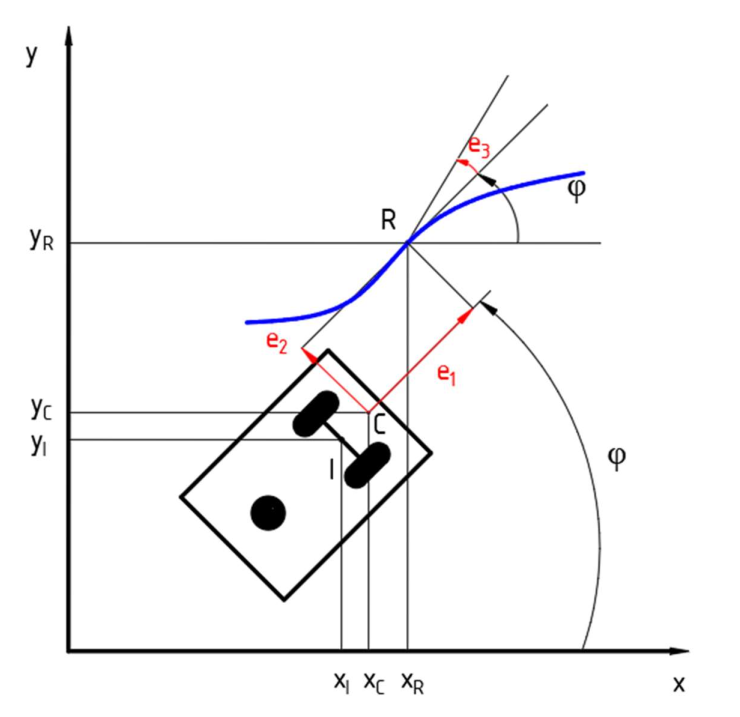
\includegraphics[width=0.55\textwidth]{pictures/chapter5/chapter5_pic1.png}
               \caption{Mô hình động học xe dò line}
               \label{kinematic_model}
          \end{figure}         
          Hình trên mô tả tọa độ các điểm cần thiết của xe trên mặt phẳng tọa độ. Trong đó
          \begin{itemize}
               \item $I(x, y)$: Trung điểm đoạn nối tâm 2 bánh chủ động.
               \item $C(x, y)$: Tâm dãy cảm biến dò line.
               \item $R(x, y)$: Tọa độ điểm tham chiếu trên đường line.
          \end{itemize}
          \hspace*{0.6cm}Phương trình động học tại $I$
          \begin{align*}
               v_{xI} &= \dot{x_I} = v \times \cos \varphi\\
               v_{yI} &= \dot{y_I} = v \times \sin \varphi\\
               \dot{\varphi_I} &= \omega
          \end{align*} 
          Đưa về dạng ma trận
          \begin{align}
               \begin{bmatrix}
                    \dot{x_I} \\
                    \dot{y_I} \\
                    \dot{\varphi_I}
                    \end{bmatrix} &= \begin{bmatrix}
                    \cos\varphi & 0 \\
                    \sin\varphi & 0 \\
                    0 & 1
                    \end{bmatrix} \begin{bmatrix}
                    v \\
                    \omega
               \end{bmatrix}
               \label{c5_e1}
          \end{align}
          \hspace*{0.6cm}Trong đó
          \begin{equation*}
               \begin{cases}
                    v = \dfrac{1}{2}(v_l + v_r) = \dfrac{r\omega_r + r\omega_l}{2} \\[0.5em]
                    \omega = \dfrac{v_r - v_l}{b} = \dfrac{r\omega_r - r\omega_l}{b}
               \end{cases}               
          \end{equation*}
          \begin{itemize}
               \item $v$: vận tốc dài của xe.
               \item $\omega$: vận tốc góc của robot.
               \item $b$: khoảng cách giữa 2 bánh xe.
          \end{itemize}
          \hspace*{0.6cm}Phương trình động học tại điểm bám line $C$
          \begin{equation}
               \begin{cases}
                    x_C = x_I + d \times \cos \varphi \\[0.5em]
                    y_C = y_I + d \times \sin \varphi \\[0.5em]
                    \varphi_C = \varphi_I = \varphi
               \end{cases}   
               \label{c5_e2}            
          \end{equation}
          \hspace*{0.6cm}Lấy đạo hàm ta được 
          \begin{equation}
               \begin{cases}
                    \dot{x_C} = \dot{x_I} - d \times \sin \varphi \dot{\varphi} \\[0.5em]
                    \dot{y_C} = \dot{y_I} + d \times \cos \varphi \dot{\varphi} \\[0.5em]
                    \dot{\varphi_C} = \dot{\varphi_I}
               \end{cases}
               \label{c5_e3}            
          \end{equation}
          \hspace*{0.6cm}Tương tự, mô hình động học tại điểm tham chiếu $R$ trên đường line
          \begin{align}
               \begin{bmatrix}
                    \dot{x_R} \\
                    \dot{y_R} \\
                    \dot{\varphi_R}
                    \end{bmatrix} &= \begin{bmatrix}
                    \cos\varphi_R & 0 \\
                    \sin\varphi_R & 0 \\
                    0 & 1
                    \end{bmatrix} \begin{bmatrix}
                    v_R \\
                    \omega_R
               \end{bmatrix}
               \label{c5_e4}
          \end{align}
          \hspace*{0.6cm}Phương trình biểu diễn sự sai lệch giữa điểm bám line $C$ và vị trí điểm tham chiếu $R$ mong muốn trên đường line
          \begin{equation}
               \begin{cases}
                    x_R - x_C = e_1 \cos \varphi - e_2 \sin \varphi \\[0.5em]
                    y_R - y_C = e_1 \sin \varphi + e_2 \cos \varphi \\[0.5em]
                    \varphi_R - \varphi_C = e_3
               \end{cases}    
               \label{c5_e5}           
          \end{equation}
          \hspace*{0.6cm}Trong đó
          \begin{itemize}
               \item $e_1$: sai số vị trí giữa điểm bám line $C$ và điểm tham chiếu $R$ theo phương vuông góc với trục hai bánh dẫn động.
               \item $e_2$: sai số vị trí giữa điểm bám line $C$ và điểm tham chiếu $R$ theo phương song song với trục hai bánh dẫn động.
               \item $e_3$: sai số góc giữa hướng của xe và hướng tiếp tuyến với sa bàn tại điểm tham chiếu $R$.
          \end{itemize}    
          \hspace*{0.6cm}Từ phương trình (\ref{c5_e5}) rút ra được hệ phương trình các sai số
          \begin{align}
               \begin{bmatrix}
                    e_1 \\
                    e_2 \\
                    e_3
                    \end{bmatrix} &= \begin{bmatrix}
                    \cos\varphi & \sin \varphi & 0 \\
                    -\sin\varphi & \cos \varphi & 0 \\
                    0 & 0 & 1
                    \end{bmatrix} \begin{bmatrix}
                    x_R - x_C \\
                    y_R - y_C \\
                    \varphi_R - \varphi_C
               \end{bmatrix}
               \label{c5_e6}
          \end{align}
          \hspace*{0.6cm}Đạo hàm 2 vế hệ (\ref{c5_e6}), khai triển và rút gọn ta thu được 
          \begin{align}
               \begin{bmatrix}
                    \dot{e_1} \\
                    \dot{e_2} \\
                    \dot{e_3}
                    \end{bmatrix} &= \begin{bmatrix}
                    v_R \cos e_3 \\
                    v_R \sin e_3 \\
                    \omega_R
                    \end{bmatrix} + \begin{bmatrix}
                    -1 & e_2 \\
                    0 & -d - e_1 \\
                    0 & -1
                    \end{bmatrix} \begin{bmatrix}
                    v_I \\
                    \omega_I
               \end{bmatrix}
               \label{c5_e7}
          \end{align}       
     \section{Tính toán thời gian lấy mẫu}
          \subsection{Tính toán thông số lấy mẫu động cơ}
               \hspace*{0.6cm}Nhóm cần tính toán thời gian lấy mẫu cho động cơ \textit{JGB37-520 333RPM} có gắn encoder với các thông số như số vòng quay sau 
               hộp giảm tốc là 333 vòng/phút, tỉ số truyền hộp giảm tốc là 1:30, 2 kênh encoder với mỗi kênh nhận 11 xung/vòng.\\
               Số vòng quay tối đa của động cơ trước hộp giảm tốc là
               \begin{equation*}
                    333 \times 30 \,\mathrm{rpm} = \dfrac{9990}{60} \,\mathrm{rev/s} = 166.5 \,\mathrm{rev/s}
               \end{equation*}
               \hspace*{0.6cm}Sử dụng 2 kênh encoder với chế độ quadrature, nghĩa là mỗi vòng encoder đếm tổng cộng $11 \times 4 = 44 \,\mathrm{xung}$.\\
               Tần số xung và thời gian giữa 2 lần đếm xung của encoder là 
               \begin{align*}
                    &f_{\text{pulse}} = 44 \times 166.5 = 7326 \,\mathrm{Hz}\\
                    &T_{\text{pulse}} = \dfrac{1}{7326} = 4.095 \,\mathrm{ms}
               \end{align*}
               \hspace*{0.6cm}Sử dụng tiêu chuẩn Nyquist, tần số tối thiểu (tương đương với thời gian lấy mẫu tối đa để khôi phục tín hiệu xung) là 
               \begin{align*}
                    &f_s \geq 2 f_{\text{pulse}} = 2 \times 7326 = 14652 \,\mathrm{Hz}\\
                    &t_s \leq \dfrac{1}{f_s} = \dfrac{1}{14652} = 0.068 \,\mathrm{ms}
               \end{align*}
               \hspace*{0.6cm}Nếu lấy mẫu theo tiêu chuẩn Nyquist, số lượng xung ở mỗi lần lấy mẫu không đủ, nhiều mẫu bị mất xung. Vì mục đích lấy mẫu động cơ không phải để tái tạo lại sóng xung encoder, mà để tính ra tốc độ trung bình của động cơ nhằm mục đích tìm hàm truyền. Nhóm sử dụng chế độ Encoder Mode của STM32 để tính toán
               số xung encoder trong mỗi lần ngắt để tính toán tốc độ động cơ làm giá trị phản hồi cho vòng điều khiển, do đó cần lựa chọn khoảng thời gian lấy mẫu sao cho số xung đọc được 
               đủ lớn để giảm thiểu sai số khi tính toán giá trị vận tốc động cơ. Nhóm lựa chọn thời gian lấy mẫu cho bộ điều khiển tốc độ động cơ là $t_s = 0.01 \,\mathrm{s}$. Số xung mà vi điều khiển đọc được trong khoảng thời gian lấy mẫu $t_s$ với tốc độ quay tối đa của động cơ là:
               \begin{equation*}
                    n = \dfrac{t_s}{T_{\text{pulse}}} = \dfrac{0.01}{\dfrac{1}{7326}} = 73.26 \,\mathrm{xung}
               \end{equation*}
               \hspace*{0.6cm}Khi chọn thời gian lấy mẫu cho động cơ là 0.01s, sử dụng encoder ở chế độ quadature, thì số vòng quay của động cơ tính trên 1 xung là:
               \begin{equation*}
                    \dfrac{60}{11 \times 4 \times 30 \times 0.01} \approx 4.54 \,\text{vòng/xung}
               \end{equation*}
               \hspace*{0.6cm}Tốc độ trung bình của xe trên cả đoạn đường là 0.5 m/s, tương ứng với vận tốc của 2 bánh xe là:
               \begin{equation*}
                    \dfrac{500}{41} \times \dfrac{60}{2 \pi} = 116.51 \,\mathrm{rpm}
               \end{equation*}
               \hspace*{0.6cm}Trong đó 41 mm là bán kính bánh xe. Số xung encoder đếm được trong khoảng thời gian lấy mẫu khi điều khiển vận tốc xe duy trì ở 0.5 m/s là:
               \begin{equation*}
                    \dfrac{116.51}{4.54} = 25.66
               \end{equation*}
               \hspace*{0.6cm}Vì số xung đếm được phải là số nguyên, do đó tại trạng thái ổn định tốc độ, số xung đếm được sẽ là 25 hoặc 26 xung, sai số xác lập là:
               \begin{align*}
                    &\dfrac{|116.51 - 25 \times 4.54|}{116.51} = 2.6 \%\\
                    &\dfrac{|116.51 - 26 \times 4.54|}{116.51} = 1.3 \%
               \end{align*}
               \hspace*{0.6cm}Sai số này nằm trong khoảng có thể chấp nhận được, do đó nhóm lựa chọn thời gian lấy mẫu cho động cơ là $t_s = 0.01 \,\mathrm{s}$.


               
          \subsection{Tính toán thời gian lấy mẫu cho bộ điều khiển bám line}
               \hspace*{0.6cm}Để tính toán thời gian lấy mẫu cho bộ điều khiển bám line, ta tính toán quãng đường tối đa mà xe di chuyển trên đoạn đường cong 
               có bán kính lớn nhất trong khoảng thời gian giữa 2 lần lấy mẫu mà vẫn đảm bảo được sai số bám line.\\
               \hspace*{0.6cm}Giả sử tâm cảm biến dò line nằm ngay tại vị trí tâm đường line tại thời điểm đầu, tại thời điểm lấy mẫu kế tiếp, với mong muốn sai số $e_2$ giữa tâm đường cảm biến 
               và tâm line không lệch nhau quá 3mm. Do đó quãng đường AB lớn nhất mà xe chạy được trước khi đạt tới sai số 3mm là: 
               \begin{equation*}
                    AB = \sqrt{OB^2 - OA^2} = \sqrt{(OA + e_{2max})^2 - OA^2}
               \end{equation*}
               \hspace*{0.6cm}Trong đó:
               \begin{itemize}
                    \item $OA$ là bán kính của đường cong.
                    \item $e_{2max}$ là khoảng sai số lớn nhất khi di chuyển trên cung.
               \end{itemize}
               \hspace*{0.6cm}Ta thấy khi $OA$ càng lớn thì khoảng di chuyển trên cung của xe càng lớn, ta tính toán với bán kính $OA = 800 \,\mathrm{mm}$
               \begin{equation*}
                    AB = 69.34 \,\mathrm{mm}
               \end{equation*}
               \hspace*{0.6cm}Để xe có thể bám được line khi vào đoạn đường cong trên thì thời gian lấy mẫu cho bộ điều khiển vị trí bám line phải thỏa:
               \begin{equation*}
                    t_{\text{đk}} \leq \dfrac{AB}{v} = \dfrac{69.34}{300} = 0.23 \,\mathrm{s}
               \end{equation*}
               \hspace*{0.6cm}$v$ là vận tốc của xe khi vào cua: $v = 300 \,\mathrm{mm/s}$. Theo sơ đồ nguyên lý điều khiển, bộ điều khiển cho xe là dạng điều khiển cascade với bộ điều khiển vị trí bám line là bộ điều khiển vòng ngoài (bộ điều khiển PID cho vận tốc động cơ là bộ điều khiển vòng trong), do đó thời gian 
               lấy mẫu và tính toán lại bộ điều khiển vị trí bám line cần đảm bảo lớn hơn thời gian lấy mẫu của bộ điều khiển PID cho vận tốc động cơ và vẫn đảm bảo điều khiển bám line đủ mượt, nghĩa là:
               \begin{equation*}
                    0.01 < t_{\text{đk}} \leq 0.23
               \end{equation*}
               \hspace*{0.6cm}Nhóm chọn $t_{\text{đk}} = 0.05 \,\mathrm{s}$.
               

     \section{Mô hình hóa động cơ}
          \hspace*{0.6cm}Thực hiện mô hình hóa động cơ, vì nhóm sử dụng driver TB612FNG để điều khiển động cơ, do đó hàm truyền tìm được bằng cách xem xét mối quan hệ giữa đầu vào giá trị xung PWM và đầu ra là tốc độ quay của trục động cơ (vòng/phút) chính là hàm truyền của cả động cơ và driver.   
          \subsection{Mô hình hóa động cơ dẫn động bánh phải}    
               \hspace*{0.6cm}Thực hiện quan sát và lấy mẫu trong 4s, với thời gian lấy mẫu là 0.01s, dữ liệu thực nghiệm thu được gồm 400 mẫu giá trị tốc độ động cơ thay đổi theo giá trị xung PWM. Do dung lượng số liệu lớn, 
               bảng dữ liệu chi tiết không trình bày trong thuyết minh mà được xử lý và thể hiện dưới dạng đồ thị đáp ứng của động cơ trong thực tế. 
               \begin{figure}[H]
                    \centering
                    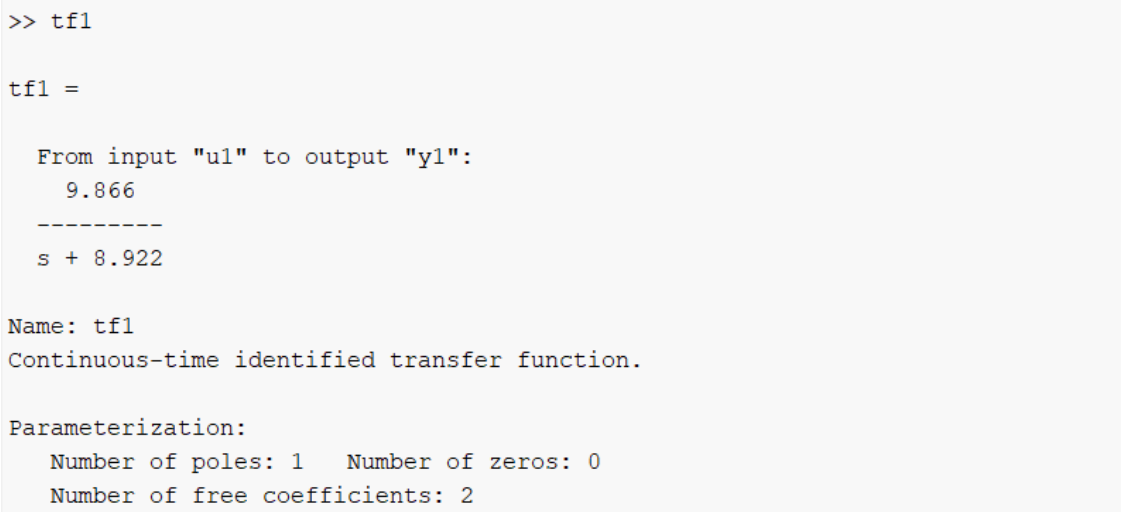
\includegraphics[width=0.8\textwidth]{pictures/chapter5/CJGB1_tf.png}
                    \caption{Hàm truyền động cơ bánh phải}
                    \label{CJGB1_tf}
               \end{figure}  
               \hspace*{0.6cm}Sử dụng Toolbox System Identification của Matlab ta có hàm truyền của động cơ bánh phải như hình (\ref{CJGB1_tf}).
               \newline
               \hspace*{0.6cm}So sánh giữa đáp ứng thực tế và hàm truyền của động cơ bánh phải
               \begin{figure}[H]
                    \centering
                    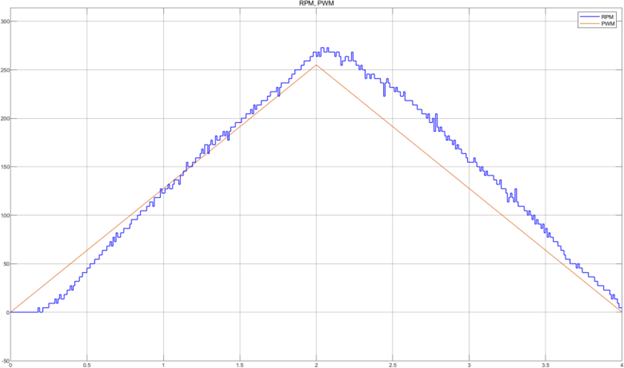
\includegraphics[width=0.75\textwidth]{pictures/chapter5/CJGB1_response.png}
                    \caption{Đồ thị đáp ứng thực tế của động cơ bánh phải theo thời gian}
                    \label{CJGB1_response}
               \end{figure} 
               \begin{figure}[H]
                    \centering
                    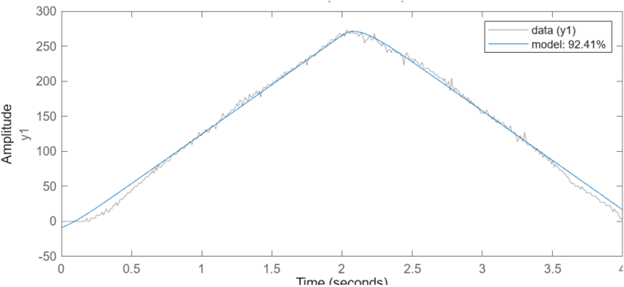
\includegraphics[width=0.9\textwidth]{pictures/chapter5/CJGB1_compare.png}
                    \caption{Đồ thị tương quan giữa đáp ứng và model hàm truyền động cơ bánh phải}
                    \label{CJGB1_compare}
               \end{figure} 
          \subsection{Mô hình hóa động cơ dẫn động bánh trái}
               \hspace*{0.6cm}Tương tự tìm hàm truyền động cơ bánh phải, dữ liệu được thu thập trong khoảng thời gian 4s với 400 mẫu giá trị, ta có đồ thị đáp ứng thực tế của động cơ bánh trái
               \begin{figure}[H]
                    \centering
                    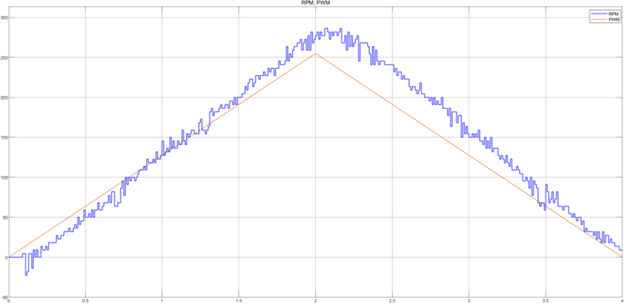
\includegraphics[width=0.85\textwidth]{pictures/chapter5/CJGB2_response.png}
                    \caption{Đồ thị đáp ứng thực tế của động cơ bánh phải theo thời gian}
                    \label{CJGB2_response}
               \end{figure}  
               Sử dụng Toolbox System Identification của Matlab ta có hàm truyền của động cơ bánh trái 
               \begin{figure}[H]
                    \centering
                    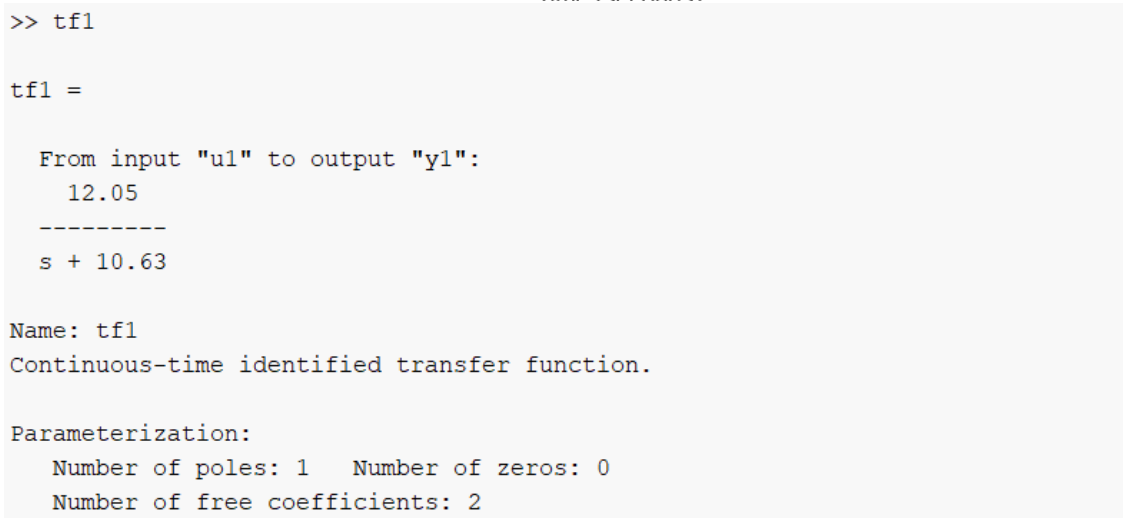
\includegraphics[width=0.8\textwidth]{pictures/chapter5/CJGB2_tf.png}
                    \caption{Hàm truyền động cơ bánh trái}
                    \label{CJGB2_tf}
               \end{figure} 
               \begin{figure}[H]
                    \centering
                    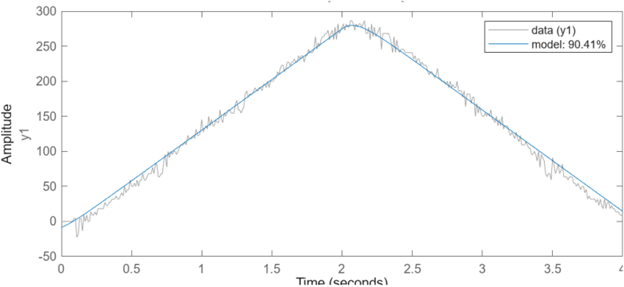
\includegraphics[width=0.9\textwidth]{pictures/chapter5/CJGB2_compare.png}
                    \caption{Đồ thị tương quan giữa đáp ứng và model hàm truyền động cơ bánh trái}
                    \label{CJGB2_compare}
               \end{figure}
               \textbf{Nhận xét:} Hai hàm truyền động cơ tìm được từ quá trình lấy mẫu
               và nhận dạng bằng Toolbox System Identification của Matlab cho thấy hàm truyền bậc I mô 
               tả khá sát hệ driver + động cơ trong thực tế. Cụ thể, đường cong mô hình và dữ liệu thực nghiệm có độ tương 
               đồng cao. Có xuất hiện sự sai lệch tại thời điểm đầu do đặc tính của động cơ có khoảng dead zone (nơi tín hiệu điều khiển nhỏ chưa thể làm quay được động cơ). Các hàm truyền thu được từ kết quả mô hình hóa này có thể được
               sử dụng làm cơ sở cho tính toán lý thuyết và triển khai thực tế bộ điều khiển vận tốc hai động cơ.
     




          


